% This file was created by matlab2tikz.
%
%The latest updates can be retrieved from
%  http://www.mathworks.com/matlabcentral/fileexchange/22022-matlab2tikz-matlab2tikz
%where you can also make suggestions and rate matlab2tikz.
%
\documentclass[]{standalone}
\usepackage{amsmath}
\usepackage{graphicx}
\usepackage[pdf]{pstricks}
\usepackage{pgfplots}
\pgfplotsset{compat=newest}
\usepgfplotslibrary{fillbetween}
%% the following commands are needed for some matlab2tikz features
\usetikzlibrary{plotmarks}
\usetikzlibrary{arrows.meta}
\usepgfplotslibrary{patchplots}
\usetikzlibrary{decorations.text}
\usetikzlibrary{shapes.multipart}

\newcommand{\logLogSlopeTriangle}[5]
{
	% #1. Relative offset in x direction.
	% #2. Width in x direction, so xA-xB.
	% #3. Relative offset in y direction.
	% #4. Slope d(y)/d(log10(x)).
	% #5. Plot options.
	
	\pgfplotsextra
	{
		\pgfkeysgetvalue{/pgfplots/xmin}{\xmin}
		\pgfkeysgetvalue{/pgfplots/xmax}{\xmax}
		\pgfkeysgetvalue{/pgfplots/ymin}{\ymin}
		\pgfkeysgetvalue{/pgfplots/ymax}{\ymax}
		
		% Calculate auxilliary quantities, in relative sense.
		\pgfmathsetmacro{\xArel}{#1}
		\pgfmathsetmacro{\yArel}{#3}
		\pgfmathsetmacro{\xBrel}{#1-#2}
		\pgfmathsetmacro{\yBrel}{\yArel}
		\pgfmathsetmacro{\xCrel}{\xArel}
		%\pgfmathsetmacro{\yCrel}{ln(\yC/exp(\ymin))/ln(exp(\ymax)/exp(\ymin))} % REPLACE THIS EXPRESSION WITH AN EXPRESSION INDEPENDENT OF \yC TO PREVENT THE 'DIMENSION TOO LARGE' ERROR.
		
		\pgfmathsetmacro{\lnxB}{\xmin*(1-(#1-#2))+\xmax*(#1-#2)} % in [xmin,xmax].
		\pgfmathsetmacro{\lnxA}{\xmin*(1-#1)+\xmax*#1} % in [xmin,xmax].
		\pgfmathsetmacro{\lnyA}{\ymin*(1-#3)+\ymax*#3} % in [ymin,ymax].
		\pgfmathsetmacro{\lnyC}{\lnyA+#4*(\lnxA-\lnxB)}
		\pgfmathsetmacro{\yCrel}{\lnyC-\ymin)/(\ymax-\ymin)} % THE IMPROVED EXPRESSION WITHOUT 'DIMENSION TOO LARGE' ERROR.
		
		% Define coordinates for \draw. MIND THE 'rel axis cs' as opposed to the 'axis cs'.
		\coordinate (A) at (rel axis cs:\xArel,\yArel);
		\coordinate (B) at (rel axis cs:\xBrel,\yBrel);
		\coordinate (C) at (rel axis cs:\xCrel,\yCrel);
		
		% Draw slope triangle.
		\draw[#5]   (A)-- node[pos=0.5,anchor=north] {1}
		(B)-- 
		(C)-- node[pos=0.5,anchor=west] {#4}
		cycle;
	}
}

\begin{document}
	
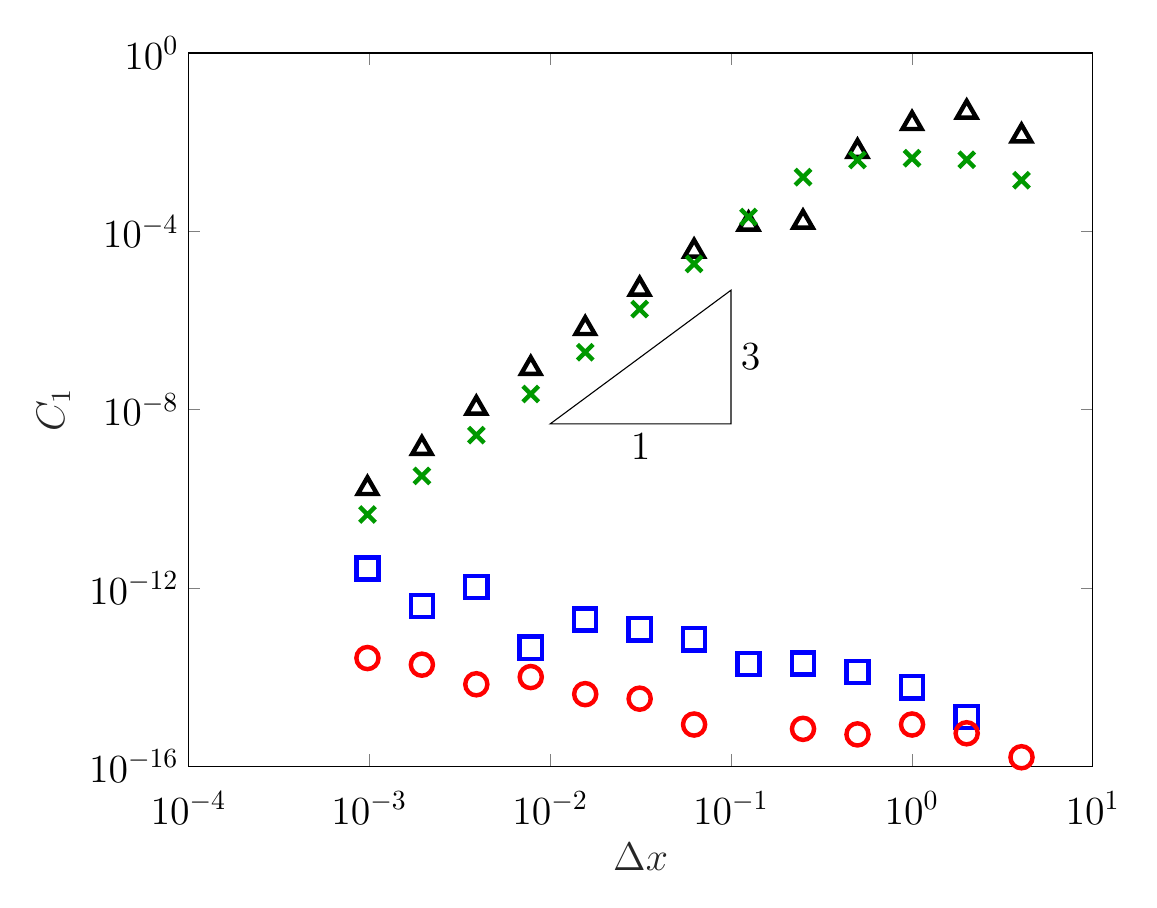
\begin{tikzpicture}
\tikzstyle{every node}=[font=\Large]
\begin{axis}[%
width=4.521in,
height=3.566in,
at={(0.758in,0.481in)},
every axis plot/.append style={ultra thick},
scale only axis,
xmode=log,
xmin=0.0001,
xmax=10,
xtick={0.0001,  0.001,   0.01,    0.1,      1,     10},
xminorticks=false,
xlabel style={font=\color{white!15!black}},
xlabel={\Large $\Delta x$},
xticklabel style = {yshift=-0.2cm},
ymode=log,
ymin=1e-16,
ymax=1,
ytick={ 1e-16,  1e-12,  1e-08, 0.0001,      1},
yminorticks=true,
ylabel style={font=\color{white!15!black}},
ylabel={\Large $C_1$},
axis background/.style={fill=white},
legend style={at={(0.03,0.97)}, anchor=north west, legend cell align=left, align=left, draw=white!15!black}
]

 \logLogSlopeTriangle{0.6}{0.2}{0.48}{3}{black};

\addplot [color=blue, draw=none, mark=square, mark size=4pt, mark options={solid, blue}]
  table[row sep=crcr]{%
4.04040404040404	0\\
2.01005025125628	1.26469734631842e-15\\
1.00250626566416	5.91646800283267e-15\\
0.500625782227785	1.31170648191206e-14\\
0.250156347717323	2.0181792818214e-14\\
0.125039074710847	1.97645382676312e-14\\
0.0625097671511174	7.05986003956983e-14\\
0.0312524415969998	1.18191233687251e-13\\
0.0156256103754053	1.94733618318875e-13\\
0.00781265259087092	4.54716767028763e-14\\
0.00390628814734519	1.04006878574139e-12\\
0.00195313453678973	3.91739960795414e-13\\
0.000976564884191612	2.74670537962459e-12\\
};

\addplot [color=red, draw=none, mark=o, mark size=4pt, mark options={solid, red}]
  table[row sep=crcr]{%
4.04040404040404	1.59261265594246e-16\\
2.01005025125628	5.49021921535001e-16\\
1.00250626566416	8.63454797755099e-16\\
0.500625782227785	5.1798795160898e-16\\
0.250156347717323	6.9065060208279e-16\\
0.125039074710847	0\\
0.0625097671511174	8.63313252603488e-16\\
0.0312524415969998	3.28059035989325e-15\\
0.0156256103754053	4.14390361249676e-15\\
0.00781265259087092	1.00144337302006e-14\\
0.00390628814734519	6.90650602082797e-15\\
0.00195313453678973	1.89928915572772e-14\\
0.000976564884191612	2.67627108307095e-14\\
};

\addplot [color=black, draw=none, mark=triangle, mark size=4pt, mark options={solid, black}]
  table[row sep=crcr]{%
4.04040404040404	0.0139102114150526\\
2.01005025125628	0.0475281802132231\\
1.00250626566416	0.0263079193573051\\
0.500625782227785	0.0062502044980619\\
0.250156347717323	0.000161273657102004\\
0.125039074710847	0.000145899216877247\\
0.0625097671511174	3.61084317581129e-05\\
0.0312524415969998	5.06317180885167e-06\\
0.0156256103754053	6.62219588576333e-07\\
0.00781265259087092	8.44641395582324e-08\\
0.00390628814734519	1.08080450489014e-08\\
0.00195313453678973	1.3588817986238e-09\\
0.000976564884191612	1.7074091989963e-10\\
};

\addplot [color=green, draw=none, mark=x, mark size=4pt, mark options={solid, green!60!black}]
  table[row sep=crcr]{%
4.04040404040404	0.00140466310963922\\
2.01005025125628	0.00403843193286285\\
1.00250626566416	0.00438205481741345\\
0.500625782227785	0.00398179294831704\\
0.250156347717323	0.00164539995543003\\
0.125039074710847	0.000209469779740006\\
0.0625097671511174	1.85576653129097e-05\\
0.0312524415969998	1.80692001550571e-06\\
0.0156256103754053	1.94482020404694e-07\\
0.00781265259087092	2.23672345353023e-08\\
0.00390628814734519	2.67643028526639e-09\\
0.00195313453678973	3.25166071376363e-10\\
0.000976564884191612	4.43630836226381e-11\\
};

\end{axis}
\end{tikzpicture}%

\end{document}